% !TEX root = mythesis.tex

%==============================================================================
\chapter{Neutrino Analysis \texorpdfstring{$60^\circ < \theta < 75^\circ$}{}}
\label{chap:DGL}
%==============================================================================
This chapter gives a brief summary of the neutrino search performed for the zenith range $60^\circ < \theta < 75^\circ$. The neutrino search is separated into different angular ranges to maximize the performance of the detector array, in this case the SD, for the search. The chapter aims to cover the expected signature in terms of measurable quantities in the Pierre Auger Observatory for the particular angular range, a description of the neutrino simulation used to develop the analysis and the reconstruction chain used to reconstruct the neutrino simulations with the Offline framework. Further, the quality cuts used are analysed in more detail, especially in the context of improving the capability of the search by the usage of MoPS and ToTd. In the end, the improvements to the neutrino detection efficiency with the inclusion of MoPS and ToTd is quantified.


\section{SD Neutrino signature \texorpdfstring{$60^{\circ} < \theta < 75^{\circ}$}{}}
\label{sec:sig_DGL}

The strategy and method to detect neutrino showers in this angular range with the SD remain the same as mentioned before in sec.~\ref{sec:EAS_nu} i.e. to try detecting showers that develop late and have more electromagnetic or "young" shower front at ground. In terms of signal in the SD array, the young shower is expected to be spread over a longer time period, typically hundreds of nanoseconds, and have a lower maximum peak compared to signal induced by older showers which are spread over tens of nanoseconds and have a higher maximum peak. A comparison of the difference between the induced SD signal from a young and old shower arriving from the same zenith angle is presented in Fig.~\ref{}. However, such differences in signals and the ability of the SD to differentiate between a neutrino induced and a proton/heavy nuclei induced shower disappear for vertical showers($\Theta < 60^{\circ}$). For vertical showers, a UHECR induced EAS does not have enough time to develop because of the limited thickness of the atmosphere. At these zenith angles a high energy UHECR induced EAS can mimic the expected young shower signature of a neutrino induced EAS at the ground. Thus, currently, the neutrino searches at the Pierre Auger Observatory are limited to zenith angles above $60^\circ$ where it is much easier to separate a neutrino induced EAS from a UHECR induced EAS. Since we are also searching for young showers which have not fully developed till they are detected at the ground, reconstructed energy cannot be used as a discrimination criterion.

To select the longer signals in the SD one of the variables that was used in erstwhile neutrino searches at Auger is the fraction of ToT-T2 triggered signals in the recorded event. As mentioned in the previous chapter this trigger is tuned to select broader signals, which for an inclined shower is evidence of a young shower. For the search presented in this thesis along with the ToT-T2, the ToTd and MoPS are also used. Both ToTd and MoPS as mentioned in sec.~\ref{sec:Sur_det_trig_new} help further increase the selection efficiency for broader signals by reducing the impact of low energy muons. These muons form the majority of the background at low zenith angles of the selected search range. Thus, these triggers are impactful in increasing the separation power for low energy ($\leq$ 1 EeV) neutrino showers. Another important variable that is used to judge the width of the signals is Area Over Peak (AoP). The AoP is defined as the ratio of the integrated signal of the station over the biggest value or peak of the signal. The AoP is calibrated in such a way that narrow or old shower signals have AoP $\sim$1 while broad/old shower signals have AoP $\geqslant$ 1. 



\section{Neutrino Simulations}
\label{sec:sim_DGL}
To characterize the neutrino search ability of the Pierre Auger Observatory Monte Carlo simulations of EASs induced by UHE$\nu$s are required. There are six possible neutrino interaction channels due to the three possible neutrino flavors with each having two possible channels (CC or NC). However, for simulations these are envisioned to be characterised by just two sets of simulations. For the NC channel since the EAS induced by three neutrino flavors has the exact same signature for our detector only $\nu_e$ NC simulations were performed for to estimate the NC contribution of all the three flavors to the final detection efficiency. 

For the CC interactions, in the case of $\nu_{\mu}$ the resulting high energy muon has a high probability of evading detection. This signature very similar to the NC interaction where the resultant secondary neutrino also carries approximately 80\% of the primary energy and probably evades detection. Thus, after taking into account the appropriate cross-section, in principle, the NC simulations can be used to also estimate the contribution of $\nu_{\mu}$ CC channel to the detection efficiency.  

In the case of $\nu_{\tau}$ CC interactions where the resulting $\tau$ especially at higher energies($\geq $EeV) can decay and also initiate a secondary shower resulting in a "double bang" like signature in the Observatory. In the context of this thesis, such signatures are not accounted for and the $\nu_{\tau}$ CC interaction is treated in the same way as the $\nu_{\mu}$ CC interaction resulting in a possible underestimation of the detection potential of the Observatory to $\nu_{\tau}$ events. A future $\nu_{\tau}$ simulation library is currently being prepared by the Pierre Auger Collaboration Monte Carlo task and could help extend this analysis in the future.

Thus, in summary, $\nu_e$ CC and NC simulations can be considered to be good approximations to estimate the contributions of all the other channels to the overall exposure of the Observatory. The simulations were produced in two parts by the Pierre Auger Collaboration Monte Carlo task based on the GAP note~\cite{gap_note_2013} and input from the author. The first part entails the simulation of the $\nu$ induced EAS in the atmosphere and the second consists of simulating the appropriate detector response for the corresponding shower. 

\subsection{Atmospheric Shower simulations}
\label{subsec:sim_EAS}
CORSIKA (COsmic Ray Simulations for KASCADE)~\cite{Heck:1998vt}, a simulation software for modelling extensive air showers in the Earth's atmosphere was used to generate the EAS initiated by a $\nu$ primary. The simulation parameters are defined through files known as input cards. An example of the input cards used to generate simulation for this analysis is provided in Appendix~\ref{sec:app_1}. The first step involved simulating the primary neutrino-nucleon interaction which is performed in CORSIKA using the HERWIG~\cite{Corcella:2000bw} code. Further, options such as CHARM to track charm secondaries are not used. Also since only $\nu_e$ simulations are simulated, the TAULEP option which handles $\nu_{\tau}$ and $\overline{\nu_{\tau}}$ is also not used. The systematic uncertainties related to the primary interaction estimator are discussed later in section~\ref{sec:det_uncert}. CORSIKA further tracks and simulates the interactions of the primary interaction products as they travel in the atmosphere toward the ground constituting the air shower. It offers a wide variety of choices regarding the hadronic interaction models it uses to simulate these interactions. For the simulations used in this study separate high and low energy hadronic interaction models were used. For energies higher than 200 GeV three high energy hadronic models QGSJETT-II.04~\cite{Ostapchenko:2010vb}, SYBILL 2.3d~\cite{Riehn:2019jet} and EPOS-LHC~\cite{Pierog:2013ria} were compared. The results of the comparison are mentioned in detail in Appendix~\ref{sec:app_2}. Since the differences between the models are not that significant for the neutrino analysis SYBILL 2.3d was chosen as the high energy interaction model. For lower energies FLUKA~\cite{Ferrari:2005zk,Battistoni:2015epi} was chosen. The systematic uncertainties arising from different models are discussed in section~\ref{sec:det_uncert}.  

To account for the curvature of the Earth which is especially important for the zenith angles studied, the EGS4~\cite{Nelson:1990sr} Monte-Carlo method is chosen to simulate the electromagnetic component of the shower. The analytical NKG method based on eq.~\ref{eq:Lateral_dist_func} which is also available but is not used for these simulations since it vastly underestimates the maximum of the electromagnetic component due to the fact it does not account for a curved atmosphere. Global Data Assimilation System (GDAS) measurements at Malargue~\cite{PierreAuger:2012jsu} were used for atmospheric profile chosen for the simulations. The magnetic field components are taken to be the default values at the Malargue site ($\mathrm{B_x = 19.52\mu T}$ and $\mathrm{B_z = -14.17\mu T}$). 

Further, since the computing times taken for shower simulations scale roughly with the primary energy, for primary energies >$10^{16}$eV these times become extremely long. Though parallel computing provides a viable solution, the technique of "thin sampling" or thinning~\cite{Hillas:1997tf} offers an alternate way to reduce the computation times while simultaneously avoiding the waste of resources. The thinning algorithm is applied to all particles below the adjustable fraction of the primary energy that emerge from an interaction. Only one of these particles is followed, and a proper weight is assigned to this particle to account for the untracked ones which are dropped based on the thinning level ($\mathrm{\epsilon_{th} = E/E_0}$). Additional information about the application and the improvements to this process can be found in~\cite{Heck:1998gr,Kobal:2001jx}. A thinning value of $10^{-6}$ is used for the simulations in this study.


The simulations were performed using the GRID technology~\cite{GRID_tech,LozanoBahilo:2012pe}. Both CC and NC showers were simulated for fixed primary energy steps of log(E/eV) = 0.5 in the range $10^{16.5}-10^{20.0}$eV. The number of simulated showers was varied depending on the Energy, atmospheric depth of interaction and the injected zenith angle. More showers were simulated at lower energies and the energy dependent numbers are tabulated in table~\ref{tab:Simulation_params}. Further, for both the interaction channels within the zenith angle range $60^{\circ}-70^{\circ}$ the neutrinos were forced to interact at fixed atmospheric depths in steps of 100 g cm$^{-2}$. The injection points both close to the ground where a neutrino shower might have a lower trigger efficiency and close to the top of the atmosphere where a neutrino induced shower might mimic one induced by a proton are rejected for the simulations. The azimuthal angle is left free and can take any value between 0$^{\circ}$ and 360$^{\circ}$. The simulated depths for each zenith angle bin are also summarised in table~\ref{tab:Simulation_params}. The values for the simulations are almost the same as used in the previous analysis~\cite{gap_note_2013} with the only change being the range for the primary energy which was simulated.

\begin{table}[h!]
  \centering
  \begin{tabular}{ |P{4.5cm}||P{0.75cm}|P{0.75cm}|P{0.75cm}|P{0.75cm}|P{0.75cm}|P{0.75cm}|P{0.75cm}|P{0.75cm}|  }
    \hline
    $\log_{10}(E/eV)$& 16.5 &17.0 & 17.5 & 18.0 & 18.5 & 19.0 & 19.5 & 20.0 \\
    Showers per ($\theta$, X) & 300 & 200 & 150 & 50 & 50 & 50 & 50 & 50\\
    \multirow{2}{*}{\shortstack{Resamplings in Offline CC \\(NC)}} & 100 & 50 & 50 & 10 & 10 & 10 & 10 & 10 \\
                            & (200) & (100) & (100) & (50) & (50) & (50) & (50) & (50) \\
    \hline
  \end{tabular}

    \bigskip
  \begin{tabular}{ |P{4cm}||P{0.75cm}|P{0.75cm}|P{0.75cm}|P{0.75cm}|P{0.75cm}|P{0.75cm}| }
    \hline
    $\theta_{MC}$  & 60$^\circ$& 63$^\circ$& 66$^\circ$& 69$^\circ$& 72$^\circ$ &75$^\circ$\\
    Interaction Depths (X) & 13    & 14 & 17 & 19 & 23 & 29\\
    Max interaction depth (g cm$^{-2}$) & 1640 & 1820 & 2040 & 2330 & 2720 & 3270\\
    Min. interaction depth (g cm$^{-2}$)& 140 & 220 & 140 & 230 & 120 & 170\\
    \hline
  \end{tabular}
  \caption{Table to test captions and labels.}
  \label{tab:Simulation_params}
\end{table}

Based on (E,$\theta_{MC}$,X) bin the number of CORSIKA showers simulated vary. Higher values were chosen for lower energies to increase the statistics since at these energies the simulated shower has a lower chance of being detected by the detector.  

After the simulation is completed CORSIKA produces a normal particle output file that contains information about the surviving particles at the ground level which is set based on the detector elevation. The file contains the relevant information such as energy, momentum, and timing all segregated for each particle based on its Particle Data Group Code~\cite{ParticleDataGroup:2024cfk}. It also produces a ".long" file that contains the longitudinal distribution of various particle numbers along with the energy deposited which is relevant analyses that use the FD. For this work, the normal particle output files were used for further processing to simulate a response in the Pierre Auger Observatory SD.

\subsection{Surface Detector Response}
\label{subsec:sim_SD_resp}

The next step required to complete the $\nu$-induced shower simulation is to generate an appropriate detector response in the SD array for each simulated atmospheric shower. This is done using the $\mathrm{\overline{Off}\underline{line}}$ framework (sec.~\ref{sec:Offline}). The framework can read in the CORSIKA output files, undo the applied thinning, simulate the Cherenkov light which will be produced as the particles travel through the WCDs and then also mimic the corresponding WCD electronics outputting the trigger and event information for each simulated shower akin to how real showers are measured at the Observatory. Each step is performed using special modules. The module sequence used to simulate the detector response for $\nu$-induced showers in this thesis is given below: 

\begingroup
  \fontfamily{cmtt}\selectfont <sequenceFile>\\
  \null\quad <enableTiming/>\\
  \null\quad <moduleControl>\\
  \null\qquad <loop numTimes="unbounded" pushEventToStack="yes"> \\
  \null\qquad \quad  <module> EventFileReaderOG </module>\\
  \null\qquad \quad  <!-- increase numTimes if you want to throw the shower\\
  \null\qquad \quad    into the array more than once -->\\
           \null \qquad \quad  <loop numTimes="5" pushEventToStack="yes">\\
           \null\qquad \quad \quad    <module> EventGeneratorOG </module>\\
           \null\qquad \quad \quad    <!-- simulation of muon background -->\\
           \null\qquad \quad \quad    <module> SdAccidentalInjectorKG </module>\\
           \null\qquad \quad \quad    <module> G4StationSimulatorOG </module>\\
           \null\qquad \quad \quad    <loop numTimes="unbounded" pushEventToStack="no">\\
           \null\qquad \quad \quad \quad          <module> CachedShowerRegeneratorOG </module>\\
           \null\qquad \quad \quad \quad          <module> G4TankSimulatorOG </module>\\
           \null\qquad \quad \quad    </loop>\\
           \null\qquad \quad \quad    <module> SdSimulationCalibrationFillerOG </module>\\
           \null\qquad \quad \quad    <module> SdPMTSimulatorOG </module>\\
           \null\qquad \quad \quad    <module> SdFilterFADCSimulatorMTU </module>\\
           \null\qquad \quad \quad    <module> SdBaselineSimulatorOG </module>\\
           \null\qquad \quad \quad    <module> TankTriggerSimulatorOG </module>\\
           \null\qquad \quad \quad    <module> TankGPSSimulatorOG </module>\\
           \null\qquad \quad \quad    <module> CentralTriggerSimulatorXb       </module>\\
           \null\qquad \quad \quad    <module> CentralTriggerEventBuilderOG    </module>\\
           \null\qquad \quad \quad    <module> EventBuilderOG                  </module>\\
           \null\qquad \quad \quad    <module> EventFileExporterOG </module>\\
           \null\qquad \quad  </loop>\\
  \null \qquad  </loop>\\
  \null \quad  </moduleControl>\\
  \null \quad  </sequenceFile>\\
\endgroup

The \textit{EventFileReaderOG} reads in the CORSIKA output file. The following steps are performed assuming an "ideal" SD array with every station operational and fully efficient within the design limits. The steps are also repeated for an individual shower between 300-10 times depending on the primary energy to further increase the statistics for each (E,$\theta$,X) bin. The first module, \textit{EventGeneratorOG}, sets the core position, time and event ID for Monte Carlo events. In this analysis similar to~\cite{gap_note_2013} the core position is only allowed to be randomized over a 5 x 5 km$^2$ area around a fixed station at the centre of the array. This is done to increase the overall simulation statistics for this study and also allows for an in depth study of how core position could impact the reconstruction which is discussed later. In the next step, the \textit{CachedShowerRegeneratorOG} reads in the list of the shower particles and un-thins each particle injecting a set of new particles based on its unique weight~\cite{Stokes:2011wf}. It can then create a list of particles for each SD station which is then passed to the next module, \textit{G4TankSimulatorOG}. G4TankSimulatorOG uses Geant4~\cite{GEANT4:2002zbu,Allison:2006ve,Allison:2016lfl} to simulate the particle trajectories in the WCD and the corresponding Cherenkov light produced by these particles. It also handles all possible absorption and reflections the light can suffer before it is measured by the PMT. Following this the \textit{SdSimulationCalibrationFillerOG} simulates the detector calibration constants described in sec.\ref{sec:Sur_det_calib} and the \textit{SdPMTSimulatorOG} takes in the information from the tank simulator and simulates a corresponding PMT signal (trace). \textit{SdFilterFADCSimulatorMTU} and \textit{SdBaselineSimulatorOG} further simulate the processing of the PMT signal by the electronics at each station with the former applying the filter response and the FADC sampling and the latter adding baseline and simulated noise to these traces. 

The next two modules decide whether the simulated event fulfils the hierarchical trigger system of the Observatory explained in sec.~\ref{sec:Sur_det_trig}. \textit{TankTriggerSimulatorOG} checks if the signal fulfils the local station criteria i.e. T1 and T2 condition. Following this the \textit{CentralTriggerSimulatorXb} further combines all the stations which fulfil the T2 criteria to form the T3, simulating the task performed by CDAS for real data. The \textit{CentralTriggerEventBuilderOG} and \textit{EventBuilderOG} then facilitate the transfer of events passing the T3 criteria from the simulation container class to the event class with the last module \textit{EventFileExporterOG} responsible for exporting all the processed showers now with the applied detector response in a file which can be used for further reconstruction.  


\section{Shower Reconstruction}
\label{sec:reco}

The event reconstruction is a necessary step before any further analysis can be performed. This procedure is developed first for neutrino simulations to enhance their identification efficiency and to study the possible background. Once fixed the reconstruction is also applied on the measured data to look for neutrino like events. Shower reconstruction is also performed within the Offline framework with a module sequence that contains a combination of some standard reconstruction modules and some specific modules developed for neutrino identification in GAP note~\cite{gap_note_2013}. The reconstruction is again performed with the help of the MC task on the GRID framework based on the particular reconstruction chain developed for neutrinos. The Module sequence used to reconstruct simulated neutrino showers is given below:

\begingroup
  \fontfamily{cmtt}\selectfont <sequenceFile>\\
  \null\quad <enableTiming/>\\
  \null\quad <moduleControl>\\
  \null\qquad <loop numTimes="unbounded" pushEventToStack="yes"> \\
    \null\qquad \quad  <!-- Event Reading and Pre-selection -->\\
    \null\qquad \quad  <module> EventFileReaderOG </module>\\
    \null \qquad \quad  <module> EventCheckerOG </module>\\
    \null\qquad \quad  <!-- SD Calibration -->\\
    \null\qquad \quad   <module> SdGainRatioCorrectorKG </module>\\
    \null\qquad \quad   <module> SdStationCheckerOG </module>\\
    \null\qquad \quad   <module> SdHistogramFitterKG </module>\\
    \null\qquad \quad   <module> SdBaselineFinderKG </module>\\
    \null\qquad \quad   <module> SdTraceCalibratorOG </module>\\
    \null\qquad \quad   <module> SdSignalRecoveryKLT </module>\\
    \null\qquad \quad  <!-- Event-selection -->\\
    \null\qquad \quad   <module> SdMonteCarloEventSelectorOG </module>\\
    \null\qquad \quad   <module> SdEventSelectorOG </module>\\
    \null\qquad \quad   <module> SdTopDownSignalSelectorUGR </module>\\
    \null\qquad \quad  <!-- Angular Reconstruction -->\\
    \null\qquad \quad   <module> SdPlaneFitOG </module>\\
    \null\qquad \quad   <module> LDFFinderKG </module>\\
    \null\qquad \quad  <!-- Post selection and export -->\\
    \null\qquad \quad   <module> DLECorrectionWG </module>\\
    \null\qquad \quad   <module> SdEventPosteriorSelectorOG </module>\\
    \null\qquad \quad   <module> RecDataWriterNG </module>\\
  \null \qquad  </loop>\\
  \null \quad  </moduleControl>\\
  \null \quad  </sequenceFile>\\
\endgroup

The sequence remains similar to the one used in~\cite{gap_note_2013} apart from the iterative development performed by the Offline developers over the years. For data reconstruction, the \textit{SdMonteCarloEventSelectorOG} is omitted from the sequence. The chain can be subdivided into three main parts which are "event reading and pre-selection," "angular reconstruction" and "posterior selection and export" which are discussed in the next few sections.

\subsection{Event reading and pre-selection}
\label{subsec:reco_presel}

The first module in this part of the reconstruction is again the \textit{EventFileReaderOG} which depending on the input format can parse the file. In the reconstruction sequence, it is used to read in either the detector response simulated file for simulations or the measurement files obtained from the SD. The \textit{EventCheckerOG} further checks if the stations in each read event have proper timing information. After this point, the FADC traces are processed with various modules to covert them to VEM units. The \textit{SdGainRatioCorrectorKG} corrects for the gain ratio for the electronics followed by \textit{TriggerTimeCorrection} which further corrects for differences in electronics especially related to timing for data over the course of its operation. The \textit{SdStationCheckerOG} further checks the station quality and appropriately sets silent stations if they do not contribute to the final trigger formation. After this point the \textit{SdHistogramFitterKG}, \textit{SdBaselineFinderKG} and \textit{SdTraceCalibratorOG} which get the calibration constants from the calibration traces, fit the baseline and convert the traces to VEM units. Further, \textit{SdStationPositionCorrection} corrects the positional differences that might arise due to faulty GPSs which is important for correct timing information, \textit{SdBadStationRejectorKG} sets known bad stations in the array to be non-operational and the \textit{SdSignalRecoveryKLT} which tries to recover signals from the saturated PMTs if any by looking at the undershoot value~\cite{Veberic:2013suc,PierreAuger:2020yab}. An extra module \textit{SdPMTQualityCheckerKG} is also used in the case of data reconstruction to estimate the quality of the detector.

The next three modules are used to fine tune the selection of signals and later events to improve both the quality of simulated and measured data to increase the efficiency of neutrino detection. The first one is the \textit{SdEventSelectorOG} which applies a basic SD event selection which is also used in other analyses. The module sets conditions based on T4, T5 and other station based parameters if appropriate. The different operations performed by the module are as follows:

\begin{description}
  \item $\bullet$~\textbf{Bottom-up Selection:} This selection helps in deciding the non-participating stations if the stations are not compatible with a planar shower front propagating at the speed of light hypothesis~\cite{gap_bottom_up}. Such stations can arise due to random noise in the array or due to random coincidences between non-air shower events with air shower events. The selection requires a minimum of three stations that fit the planar front of the shower within lenient time tolerances. It also removes isolated stations by checking the distances to nearest neighbours. Although the selection is applied, it is not very effective for inclined showers(>$60^{\circ}$) since the showers above these angles are not geometrically compact. Thus, this selection is supplemented with an extra top-down selection implemented in \textit{SdTopDownSignalSelectorUGR} which is discussed later. 
  \item $\bullet$~\textbf{T4 and T5 trigger:} The module also calculates the T4 and T5 criteria discussed in sec.~\ref{sec:Sur_det_trig_array}. It then further discards events if they do not fulfil these criteria. In this study, the T4 criteria was not used but a stringent 6T5 criteria was required for the selection. 
  \item $\bullet$~\textbf{Lightning Rejection:} The lightning events can be detected in the SD stations by looking for an oscillatory signal in the FADC trace of all three PMTs~\cite{2017AGUFMAE31A..06C}. For this analysis, if any lightning like signal is detected in any one of the stations the whole event is rejected from the analysis. 
  \item $\bullet$~\textbf{ToTd and MoPS trigger:} The module can also silence particular triggers before applying the selection. This feature is used to produce two sets of reconstruction files one with the triggers turned off and one with them turned on to check the impact of the new triggers. This can impact the number of events fulfilling the 6T5 conditions and thus the overall number of events which can be seen later.    
\end{description}

The \textit{MonteCarloEventSelectorOG} further removes stations with distance in shower plane coordinates smaller than the inner radius used in the CORSIKA simulations. It also removes dense stations i.e. virtual stations which are sometimes used for MC studies since these are not representative of the regular SD array. 

The \textit{SdTopDownSignalSelectorUGR} is a module developed specifically to carry out a top-down selection and accidental signal rejection for neutrino like events. A summarised overview of what this module aims to accomplish is given next with a detailed description of the module already published in~\cite{}(Billor?). The Top-down procedure is applicable for both the simulations and measured data whereas the accidental signal treatment is only applied for measured data. The procedure is based on~\cite{} and~\cite{}. Top-down selection requires a minimum of three stations with the shower front time tolerance compatibility dependent on the zenith angle. If the fit does not converge stations are successively removed and re-tested until a satisfactory fit is achieved. At the end of the procedure stations which do not contribute to the final fit are rejected while the others are marked as candidate stations. Further, the Top-Down procedure also takes into account the individual traces and uses the shape for 3-fold topologies. It also rejects isolated signals akin to the Bottom-up selection but with larger tolerances to account for the wider footprint of inclined events. The module also applies an accidental signal rejection procedure before the top-down procedure is applied to account for the atmospheric muon background. The atmospheric muons and also local showers can either trigger isolated stations or even real event stations affecting the start times and in turn the zenith angle reconstruction. This miss-reconstruction can either cause problems with the fitting of the top-down procedure and can also lead to non-neutrino like or background events past the analysis cuts affecting the overall neutrino detection efficiency. The module discards stations with total signals below 3 VEM which rejects the muonic background which typically peaks at 1 VEM. The discarding procedure is implemented only till the minimal number of stations present in the event is below 6.

Since the parameters of the module were evaluated without the consideration of MoPS and ToTd especially for the segment selection procedure slight changes were made to the module. The segmentation procedure was not applied to the stations which had a MoPS/ToTd trigger. These stations were only subjected to the top-down selection procedure. Some more details about this choice are presented in Appendix~\ref{sec:app_3}. Further, the accidental station cut was lowered till the minimum number of stations present in the event are below 5 compared to 6 to account for the increased number of stations expected with the inclusion of new triggers. This was done after the partial unblinding of the test sample and is described in more detail in sec.~\ref{subsec:unblind_20}. These changes were only implemented for the sample where the new triggers are included and the sample where they are not remains unchanged. 

\subsection{Angular Reconstruction}
\label{subsec:angular_reco}

The angular reconstruction forms the basis for neutrino detection using the SD especially since for inclined neutrinos the primary energy estimation algorithms typically used for CRs at the Pierre Auger Observatory become unreliable. The angular reconstruction is performed by the \textit{SdPlaneFitOG} and \textit{LDFFinderKG}. The primary energy estimation using the SD is typically done using the \textit{LDFFinderKG} which fits a lateral distribution function to the SD signal based on the NKG approximation. The NKG approximation is typically inaccurate for inclined showers above a zenith of $60^{\circ}$ thus alternate methods based on muon maps are used for CR inclined showers. These also fail for neutrino induced showers which in our detection scenario usually have a large electromagnetic component. Thus, without a reliable energy reconstruction, angular reconstruction becomes vital for neutrino induced shower detection at the SD. A summary of the method and the procedure is presented below based on a detailed description which can be found in~\cite{PierreAuger:2020yab}. 

The angular reconstruction procedure uses the timing information from the stations to fit either a plane or a spherical shower front. The axis of shower $\hat{a}$ is initially assumed to intersect the ground at some time using a signal weighted barycenter $x_b$ and bary-time $t_b$ of selected stations located at $x_i$ with start time $t_i$ given by :

\begin{equation}
  \vec{x_b} = \frac{\sum_{i} S_i x_i}{\sum_{i} S_i} \quad \text{and} \quad t_b = \frac{\sum_{i} S_i t_i}{\sum_{i} S_i}
\end{equation}

The choice of the weights taken as $\sqrt{S} $ with $S$ being the signal of the stations has been previously evaluated using Monte-Carlo studies to give the best results. The barycenter also serves as the first estimate of the impact position of \textit{shower core} at the ground but is later estimated more accurately. The shower core is assumed to be moving in the $-a$ direction. Under the plane-front assumption the particles in the shower front move in a plane perpendicular to the shower axis ($shower plane$) with the same speed as the core of the shower which is the speed of light, c, the time, t($\vec{x}$) when the shower plane passes through some chosen point, $\vec{x}$ (e.g. a station on the ground) can be inferred through a simple projection onto the shower axis as,
\begin{equation}
  ct(\vec{x}) = ct_b - (\vec{x}-\vec{x_b})\cdot \hat{a}
\end{equation}

Assuming a minimal change in altitude which is true for the SD location and precise knowledge of station locations the deviations in estimating the geometrical shower parameters can be due to the uncertainty of the observed start times $\sigma_t$. Thus, the following function needs to be minimized to fit the model for the measured signal start times 
\begin{equation}
  \chi^2 = \sum_{i} \left(\frac{t_i - t(\vec{x_i})}{\sigma_{t_{i}}}\right)^2
\end{equation}

\todo{Add the schematics}

% \begin{figure}[t!]
%   \centering
%   \subcaptionbox{SChematic of plane-front approximation  \label{sub:fig:plane_fit}}{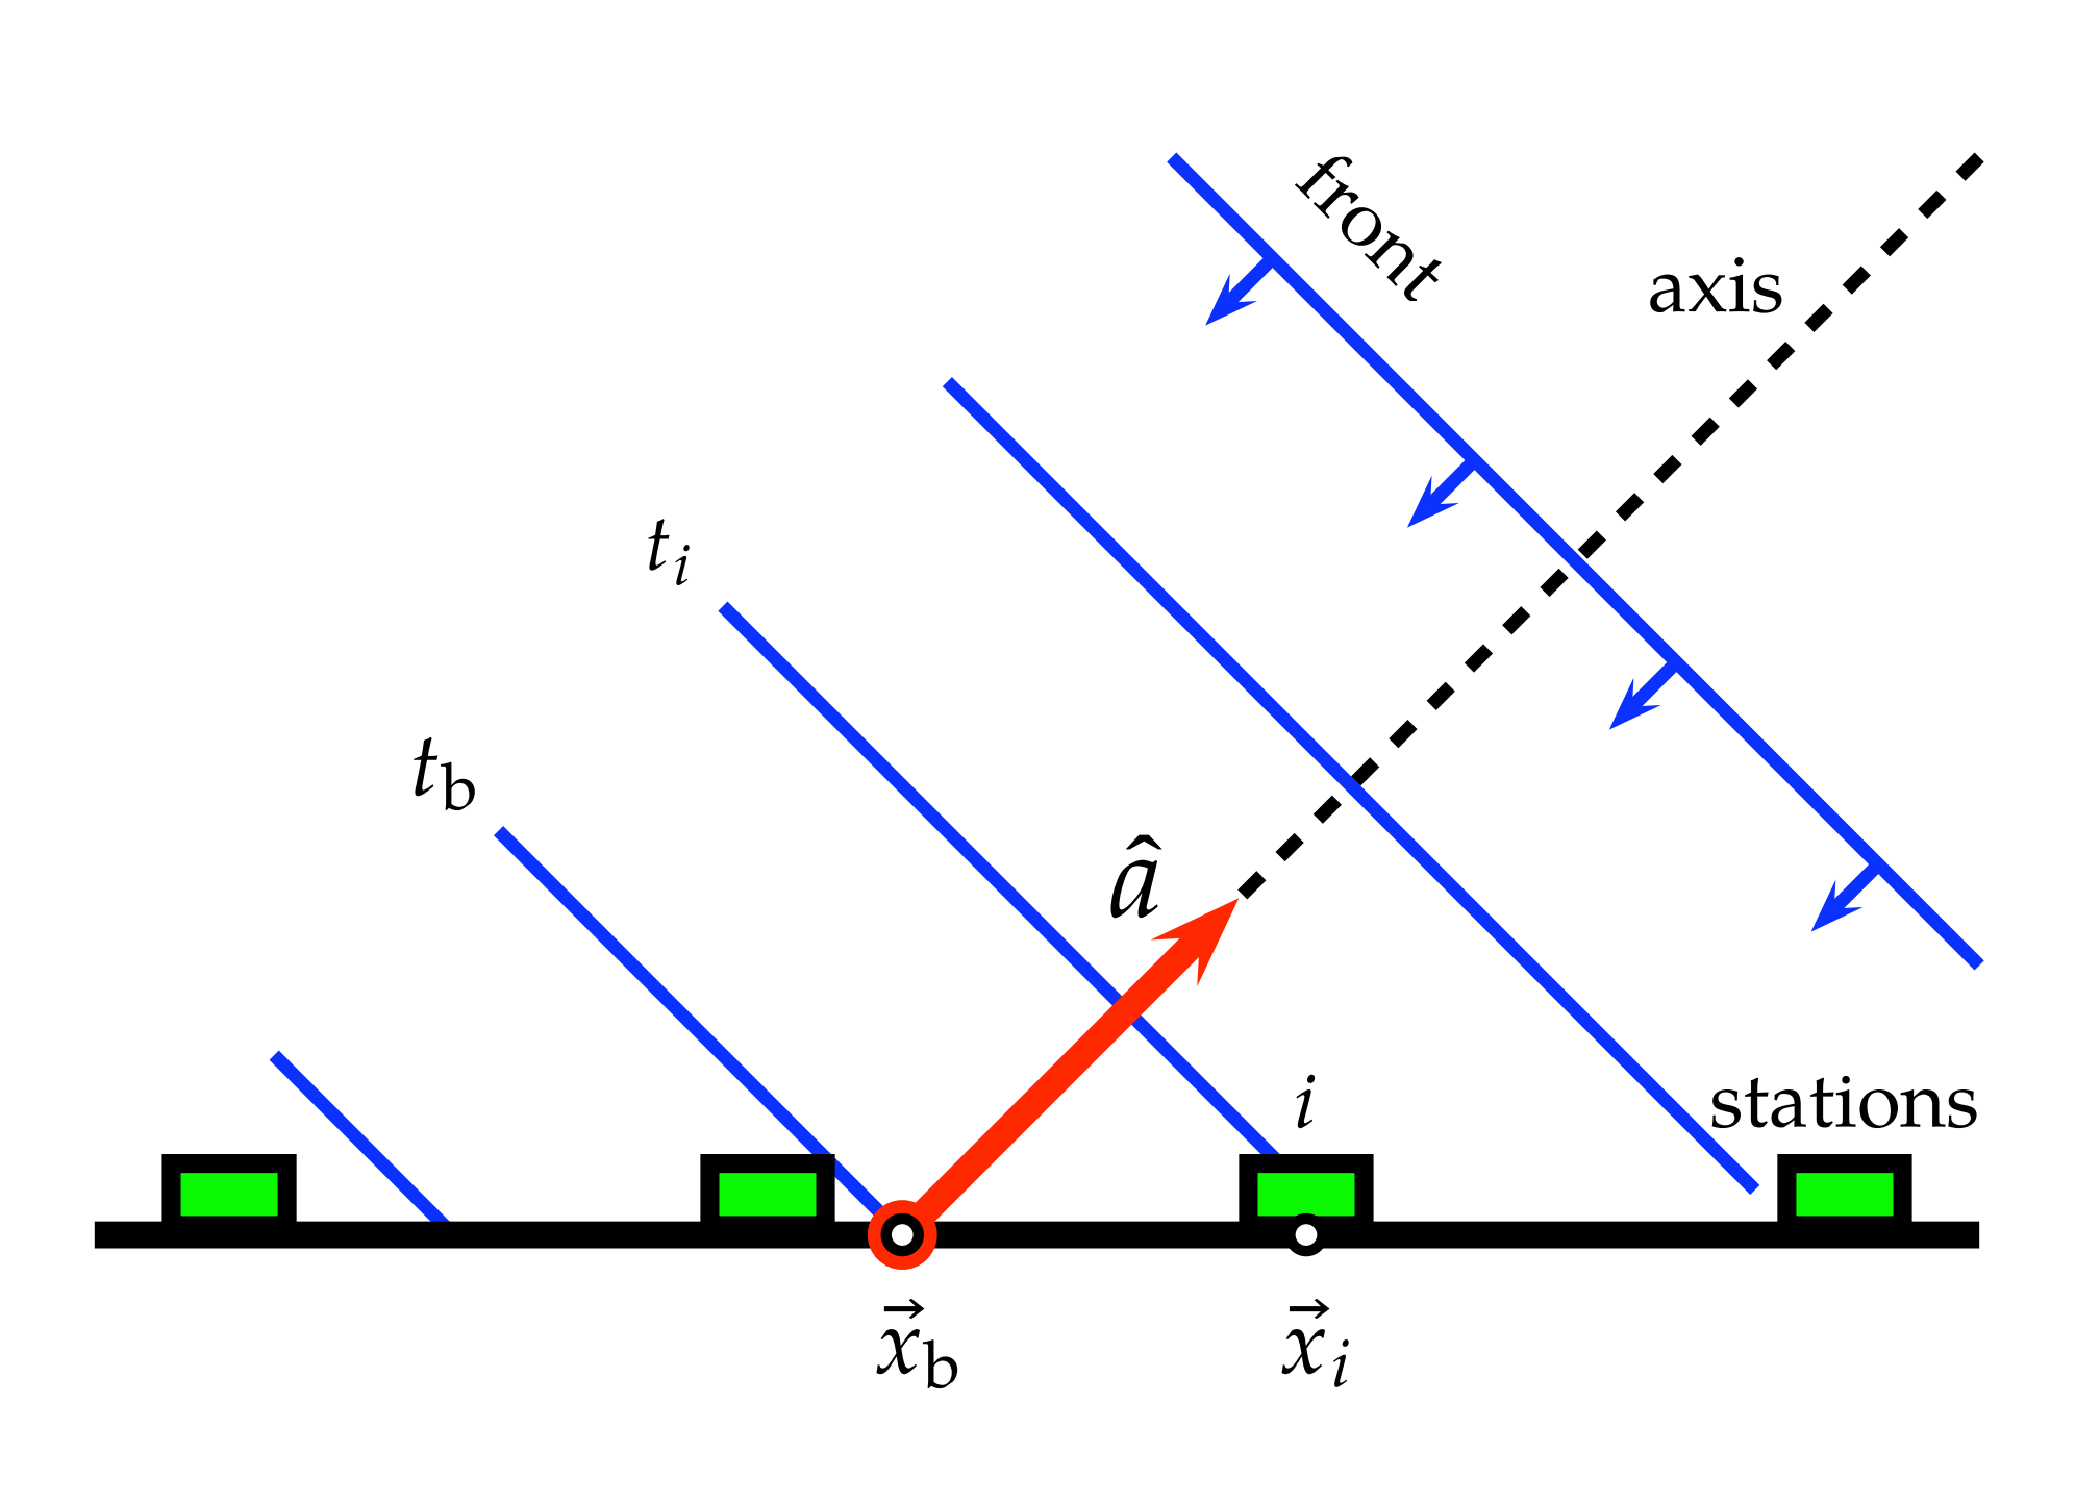
\includegraphics[width=.45\linewidth]{thesis_figures/Nu_analysis/Plane_fit.pdf}}
%   \hfill
%   \subcaptionbox{2C$_1$\&3C$_2$\&4C$_4$\label{sub:fig:T3_config_2}}{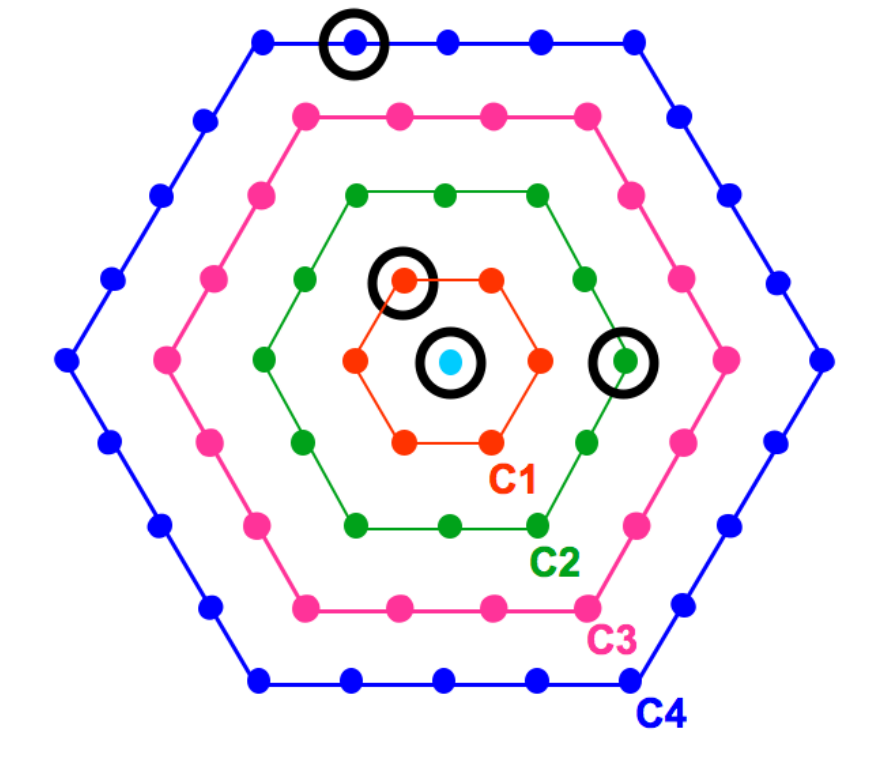
\includegraphics[width=.45\linewidth]{thesis_figures/Setup/T3_config_2.png}}
%   \caption{Example of two possible T3 configurations. Taken from~\cite{PierreAuger:2010zof}}
%   \label{fig:T3_config}
% \end{figure}
\begin{figure}[h!]
  \centering
  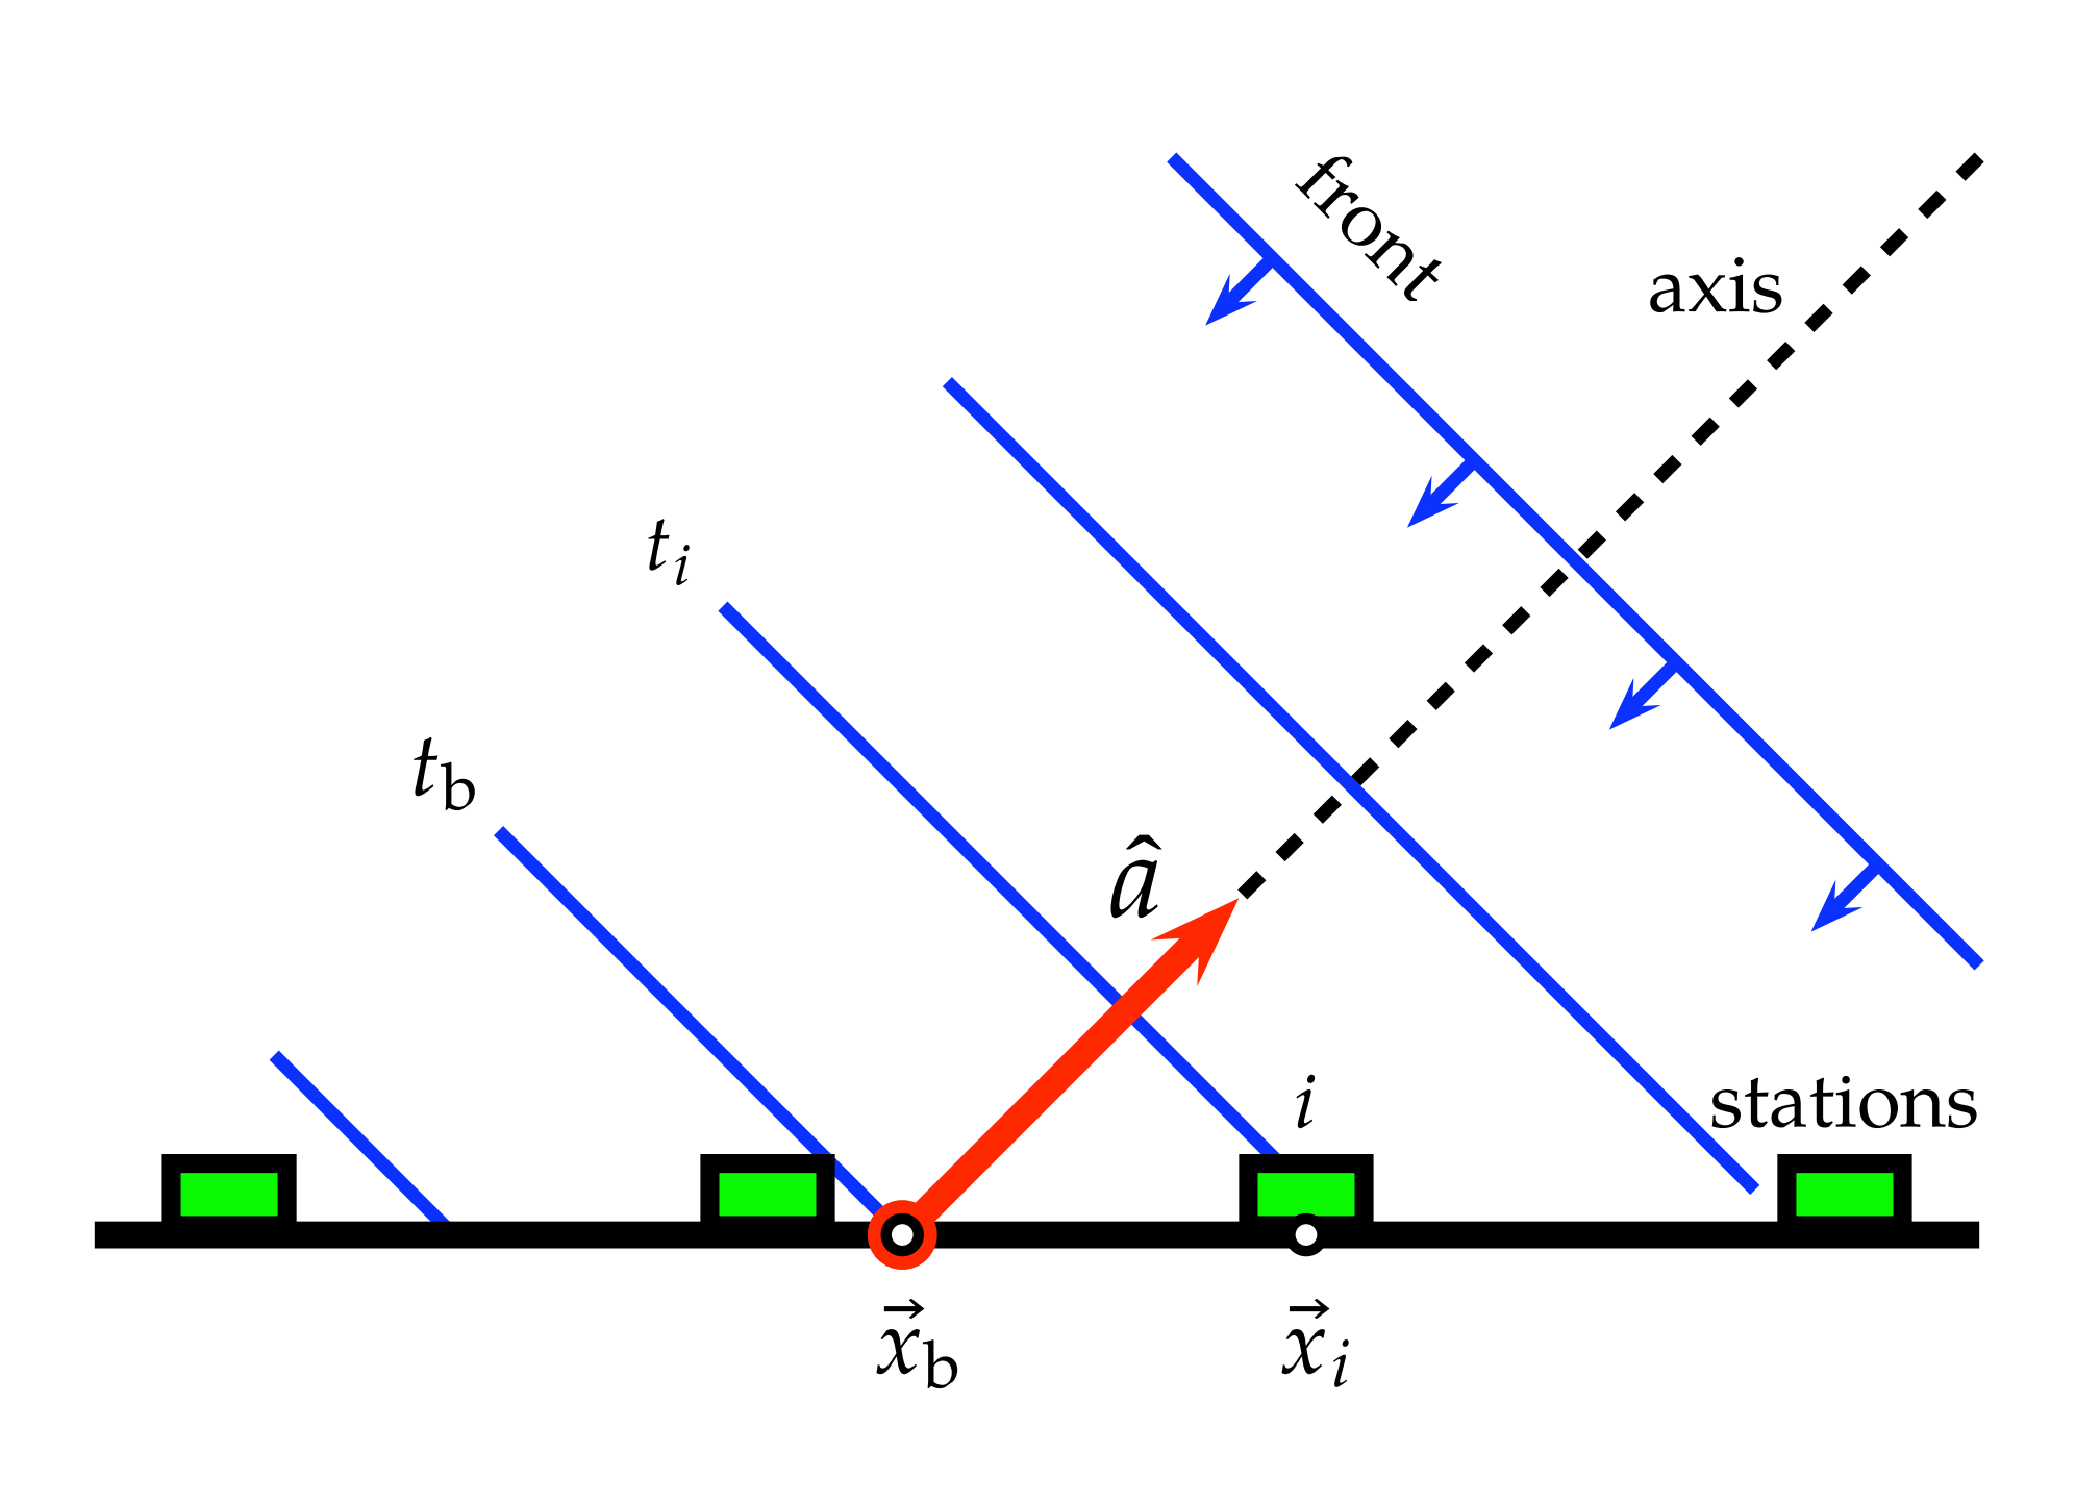
\includegraphics[width=\textwidth]{thesis_figures/Nu_analysis/Plane_fit.pdf}
  \caption{Schematic of plane-front approximation. Taken from~\cite{PierreAuger:2020yab}}
  \label{fig:Plane_fit}
  \end{figure}

where $t_i$ are the start time of the signals of station i located at $x_i = \vec{x} - \vec{x_b}$. The minimization of the $\chi^2$ is performed using MINUIT~\cite{James:1975dr}. For the start time variance determination the standard model described in~\cite{PierreAuger:2020yab} is used. Modifications for new triggers have been suggested in~\cite{}(Coleman thesis), but these have not yet been approved by the Collaboration for wider use. Replacing the axis with $a =(u,v,w)$ and the station coordinates with $x = (x,y)$ (ignoring altitude z). Adding the constraint $u^2 + v^2 + w^2 = 1$ the $chi^2$ can be easily solved. The solution only fails if the stations used while fitting have a linear dependence (three stations in a line) but for higher station multiplicity this is highly improbable, especially for the theta range explored for the DG$\mathrm{_{low}}$ channel.

\begin{figure}[h!]
  \centering
  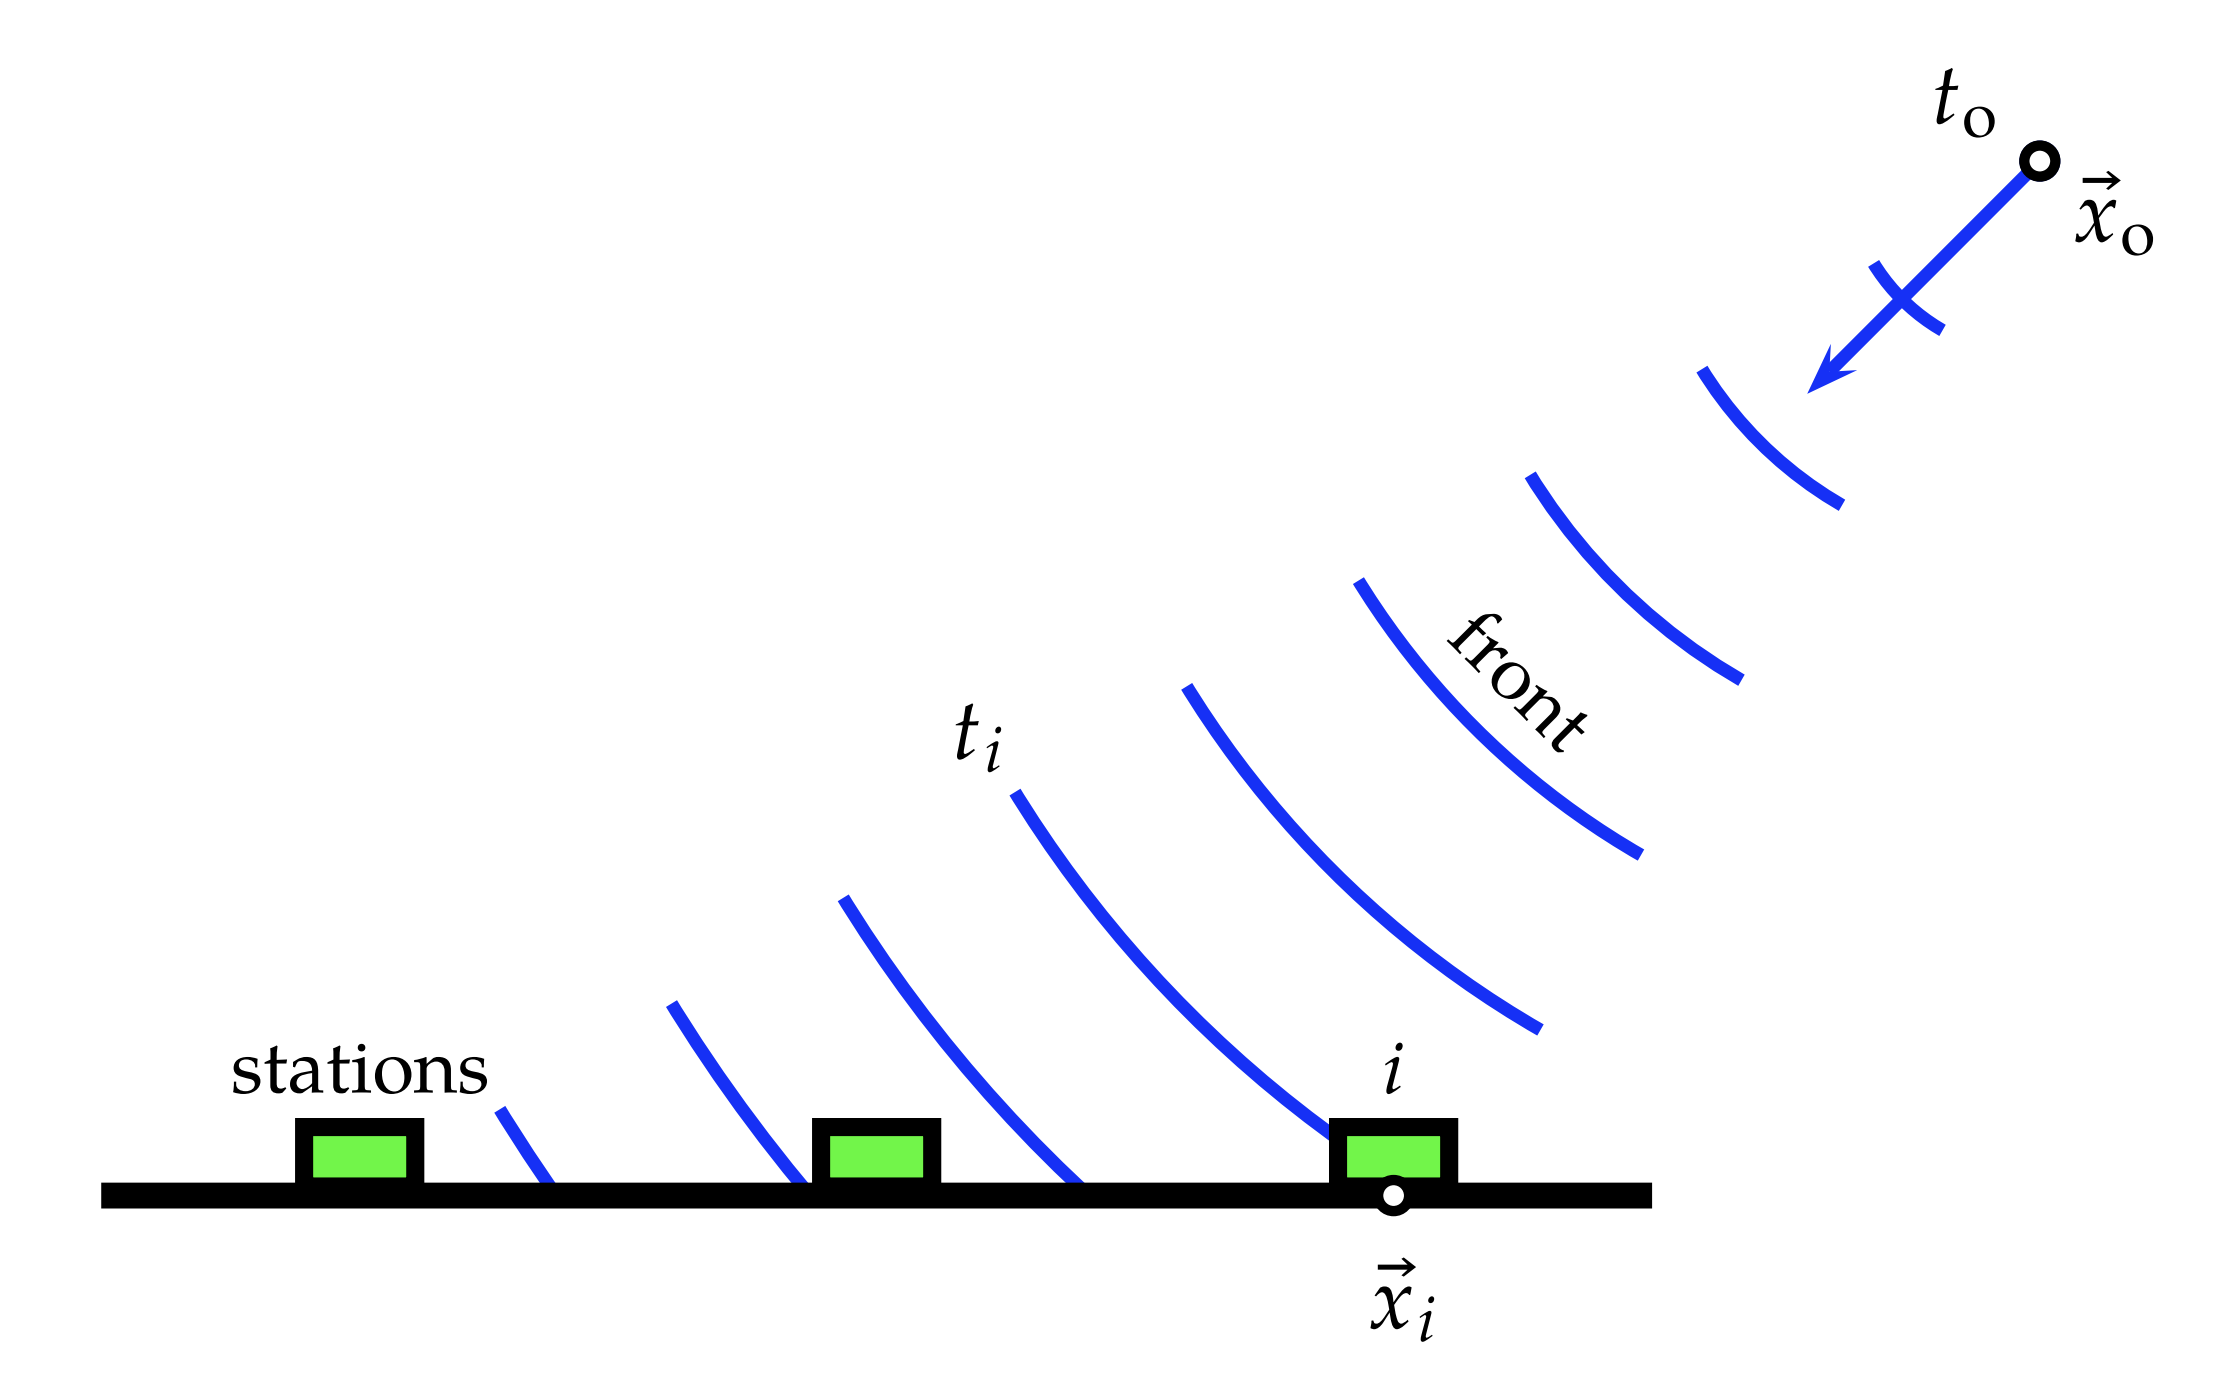
\includegraphics[width=\textwidth]{thesis_figures/Nu_analysis/Spherical_fit.png}
  \caption{Schematic of spherical-front approximation. Taken from~\cite{PierreAuger:2020yab}}
  \label{fig:Spherical_fit}
\end{figure}

Another shower front estimation technique based on a curved shower front approximation is also used to fit the measured stations. The reconstruction called the $Observer$, assumes the shower development starting at time $t_o$ from a point of origin $x_o$ propagating toward the ground as a concentrically expanding sphere with the speed of light, $c$. The arrival time of the shower front at point $\vec{x}$can thus be estimated as:
\begin{equation}
  t(\vec{x}) = t_o + \frac{|\vec{x}-\vec{x_o}|}{c}
\end{equation}

As can be seen by the equation, the spherical fit is decoupled from any prior knowledge of the shower core or the shower axis. It is only dependent on the point of origin. Quantities such as the shower axis can be determined later when the impact point, $\vec{x_c}$ has been estimated as $ \hat{a} = (\vec{x_o} -\vec{x_c})/ (\vec{x_o}-\vec{x_c})$. The expected solid angle differences between the two fits are of the order of half a degree. The curvature shower front fit is only used for station multiplicities greater than five. This is so because for lower station multiplicities the degrees of freedom are not enough to solve for the shower-front curvature. A side by side comparison for an event for both plane fit and spherical fit is shown in fig.~\ref{}.

\subsection{Posterior selection and Export}
\label{subsec:reco_possel}

The last part of the shower reconstruction chain includes the application of the \textit{SdEventPosteriorSelectorOG} module which computes the 6T5 \textit{posterior} trigger differing from the 6T5 criteria mentioned earlier. The 6T5 posterior requires the 6 stations in the first crown from the nearest station to the reconstructed shower axis to be active or alive during the event. The events which do not pass this criterion are rejected. The last module \textit{RecDataWriterNG} exports all the relevant information to ADST~\ref{sec:ADST} files. In the case of reconstructed simulations, both the simulated and reconstructed information are stored while for measured data only the reconstructed information is stored.

\section{Reconstructed \texorpdfstring{$\nu$}{} simulations}
\label{sec:reco_possel}
This section includes some sanity checks to check and verify the quality of the $\nu$ simulations. Fig shows the Efficiency of the reconstructed showers as a function of the zenith angle and the slant depth. The next figure shows the frequency of reconstructed events based on the core position. The non-uniform distribution with minimal events for core positions close to the stations can be explained arising due to two reasons. The first is the removal of stations if the PMTs for the particular station are saturated. This saturation can occur for stations very close to the core. The second reason  
\todo{Expand with plots}
\textit{What to include here? Theta distributions, AoP distribution comparisons, Core position distributions, Residuals, Xmax distributions etc.}

\section{\texorpdfstring{$\nu$}{} selection}
\label{sec:nu_sel}
This section tries to describe the decisions made to select $\nu$ induced air showers. The selection is optimized and evaluated on the above-mentioned neutrino simulations and a part of the measured data is used as an estimate for the expected background. Since a \textit{blind search} strategy is envisioned for the search. The rest of the measured data forms the \textit{search sample} and will be used to look for neutrino like events during the \textit{unblinding}. 
In the first part the selection used to identify $\nu$ showers is described in more detail. The selection consists of some pre-selection cuts applied to enhance the reconstruction quality of the selected events followed by a Fisher Linear Discriminant~\cite{Fisher_illustrative} based on experimental observables which is the main criteria of differentiation between a $\nu$ induced air shower and background.  
In the second part, the performance of the selection is further evaluated based on temporal changes such as ageing in the surface detector and the neutrino detection efficiency is quantified. Comparisons to previously used selection are also presented especially in the context of the performance improvements achieved by using new triggers for neutrino detection.

\subsection{Samples Used}
\label{subsec:nu_sel_samp}

As mentioned above to devise an efficient neutrino selection good quality training samples for both signal and background are required. Monte-Carlo simulations described in~\ref{sec:sim_DGL} are used for the signal sample. For the background sample a portion of real data (20\%) is used. Due to the low flux prediction of neutrinos a large portion of the measured data if not all is expected to be nucleonic air showers. Simulated showers could also serve as background sample, but this is not done to due to the following reasons. For the energies that are investigated in this search the high uncertainties observed for the air shower simulations, particularly due to hadronic interaction models could lead to errors. Further, the simulations are still incomplete i.e. they tend to sometimes ignore some physical processes and also do not account for all the possible and sometimes unpredictable detector effects which could be important for the neutrino search. Using measured data as background is advantageous here as it already contains all the possible effects. Also, due to the vast parameter space looked at for the neutrino search such a simulated background sample would require huge amount of computing resources. 

The number of 20\% of the measured data sample for the time period 2014-2021 is arrived at to keep the search sample i.e. the rest 80\% large enough to look for neutrinos but still have enough events in the training sample for Fisher analysis. The training data for the time period corresponds to 1.29+-?? years of the continuous measurement of a full array composed of 1420 T5 hexagons. Periods of instability or large outages marked as "BadPeriods" are rejected. The events are chosen at random across the time period from the full sample of measured data by only taking those events where the Auger SD event ID is divisible by 5. The time period is chosen to be starting from the year 2014 since by this time the array had full coverage of MoPS and ToTd. The end date of December 31, 2021 was decided in discussions with the collaboration as the end of Phase 1 of data taking of the Pierre Auger Observatory since after this point significant changes were made to the electronics of the Surface Detector tanks as a part of AugerPrime activities as previous mentioned in sec.~\ref{sec:Aug_prime}.

The remaining sample which consists of events with SD ids not divisible by 5 which is 80\% of the full sample was unblinded in two parts. A 20\% test sample was unblinded first to check if there was any need for further optimisation of the analysis and the rest 60\% constituted the search sample and was used to look for neutrino candidates.   

\begin{table}[h!]
  \centering
  \begin{tabular}{ |P{3cm}||P{8cm}| }
    \hline
       \multicolumn{2}{|c|}{Samples Used} \\
       \hline
       \multirow{2}{*}{\shortstack{MC $\nu$\\ training sample}} & Simulated events \\
                                  & Detailed info tab.~\ref{tab:Simulation_params} \\
    \hline 
    \multicolumn{2}{|c|}{Analysed data period -  01.01.2014 till 31.12.2021} \\
    \hline
    \multirow{3}{*}{\shortstack{Background\\ \textit{training} sample}} & 20\% analysed data \\
                                  &  1.29 $\pm$ .. yr of full Auger equivalent exposure \\
                                  & (SD event IDs divisible by 5) \\
    \hline
    \multirow{3}{*}{\shortstack{Signal\\ \textit{search} sample}} & 20\% + 60\% analysed data \\
                                  &  6.45 $\pm$ .. yr of full Auger equivalent exposure \\
                          & (SD event IDs non-divisible by 5) \\               
    \hline
  \end{tabular}
  \caption{Table to test captions and labels.}
  \label{tab:samples_info}
\end{table}
\subsection{Pre-selection Cuts}
\label{subsec:nu_sel_preselcut}

The pre-selection cuts are applied based on the unique properties of "young" neutrino like showers in comparison to older nucleon like showers. The cuts are the same as used in GAP 2013 with a slight modification to include MoPS and ToTd. These pre-selection cuts are applied in the same way to both the neutrino and background training samples. 
\begin{description}
  \item ~\textbf{Inclined Shower Selection:} This cut aims to select showers which fall in the given angular window. The reconstructed zenith of each event is required to be in the range 58.5$^{\circ} < \mathrm{\theta_{rec} < 76.5^{\circ}}$. The range is extended by 1.5$^\circ$ on both sides in comparison to the simulated values from the simulations to account for the angular resolution of the detector. Further, the error on the reconstructed angle, $\mathrm{\Delta \theta_{rec}}$ is required to be smaller than $3^\circ$ to ensure the quality of angular reconstruction. The efficiency of this cut is found to be ... for CC(NC) neutrinos. The angular distribution of the background sample is shown in fig.~\ref{}.
  \item ~\textbf{Fiducial Quality Cut} This cut also remains unchanged when compared to the previous analysis. The main aim of the cut is to ensure that the shower core for the selected event is completely contained inside the array and the stations which are used for the analysis of the event are operational. This is ensured by requiring the event to satisfy the 6T5 trigger condition. The efficiency of the cut is 100\% for the neutrino simulations by design and for the background sample this cut leads to a reduction of ... as shown in fig.~\ref{}   
  \item ~\textbf{Young Shower Selection} This cut tries to ensure the selection of events with a high electromagnetic component at ground. For this purpose events with stations having FADC traces spread in time need to be selected. As mentioned previously ToT, ToTd and MoPS triggers being more sensitive to the presence of high electromagnetic component can be used for this young shower selection. This cut ensures that more than 75\% of stations in the T5 hexagon satisfy the ToT/MoPS/ToTd condition. the 75\% fraction is calculated overall per event basis and the hexagon could have stations with mixtures of these triggers. The cut retains most of the neutrino events and at the same time is highly effective in rejecting background especially for high angles as shown in the fig.~\ref{}.
  \item ~\textbf{Angular Fit Quality} A few erroneous events were discovered to have a bad geometric fit. This problem though discovered with the analysis with new triggers has always affected the neutrino analysis. To mitigate this problem a fit quality cut based on the goodness of the geometry fit was devised. The cut only accepts events which have a goodness of geometrical fit less than 200. The efficiency of the cut is $\sim$99\% for the neutrino simulations and for the background sample this cut leads to a reduction of <0.1\% of events. The goodness of fit comparison for background and neutrinos is shown in fig.~\ref{}. Although the cut has minimal impact it, it ensures that one of the fundamental pillars of the analysis i.e. the geometry of the shower especially the zenith angle is well reconstructed.
\end{description} 

\subsection{Fisher linear discriminant analysis}
\label{subsec:nu_sel_fisher}
The last step for the $\nu$ selection and identification involves Fisher Discriminant Analysis (FDA) also known as Linear Discriminant Analysis(LDA). This is a statistical method used to find a linear combination of features i.e. Fisher polynomial that characterizes and separates the two classes, in our case, signal and background distributions. The goal of FDA is to find a projection that maximises the distance between the projected class means while minimising the variance within each class. This ensures that the classes are well-separated in the reduced space. Mathematically, if we have a signal class represented by $X_s$ with mean $\mu_s$ and a background class $X_b$ with mean $\mu_b$ then the optimal discriminating hyperplane represented by $w$ can be found by solving the equation $S_B w = \lambda S_W w$. The solution is the eigenvector corresponding to the largest eigenvalue $\lambda$. $S_B$ is called the between-class matrix and represented as follows: 

\begin{equation}
  S_B = \sum_{i = X_s,X_b} n_i (\mu_i - \mu)(\mu_i - \mu)^T
\end{equation}
with $\mu = \frac{n_s \mu_s + n_B \mu_b}{n_s + n_b}$ is the overall mean 

The between class matrix $S_W$ is given as
\begin{equation}
  S_W = \sum_{i = X_s,X_b} \sum_{j = n_s,n_b } (x^{(i)}_j - \mu_i) (x^{(i)}_j - \mu_i)^T
\end{equation}

After finding the weight vector, the projected data for each sample is given as $z_i = w^Tx_i$, $z_i$ from here on is referred to as Fisher value, $\mathcal{F}$. The elements of the normalised transposed weight vector are called Fisher coefficients. The method has been implemented in a standalone python program with the help of~\cite{JaimeAlvarezMuniz_conversation} and has been verified with the inbuilt LDA module of python~\cite{scikit_Learn} with both results agreeing within 0.01\%. 

\subsubsection{Fisher polynomials and training}
\label{subsubsec:nu_sel_fisher_training}
It is really important to find the correct features or variables to train the algorithm to achieve the best possible separation. Various combinations of input features were tested and evaluated based on the level of separation along with the shape of the tail of the background description which is important for the cut evaluation procedure. As mentioned before AoP will remain the primary feature used for discrimination. It was also shown in~\cite{gap_note_2013} that for the DG$\mathrm{_{low}}$ channel AoPs of the earliest stations closest to the core provide the best level of discrimination between data and background. This also visualized in figs.~\ref{}. Further, the zenith angle range for the search, 58.5$^\circ < \theta < 76.5^\circ$ is subdivided into five sub-regions similar to~\cite{gap_note_2013} as shown in fig~\cite{}. This is done to incorporate shower age while training the Fisher polynomial. The first four angular regions are $3^\circ$ each whereas the last region is $6^\circ$. This is due to the small amount of statistics expected for higher angles which required a larger window size. For each angular window the Fisher polynomial is trained separately to maximise the analysis performance. 

\begin{figure}[h!]
  \centering
  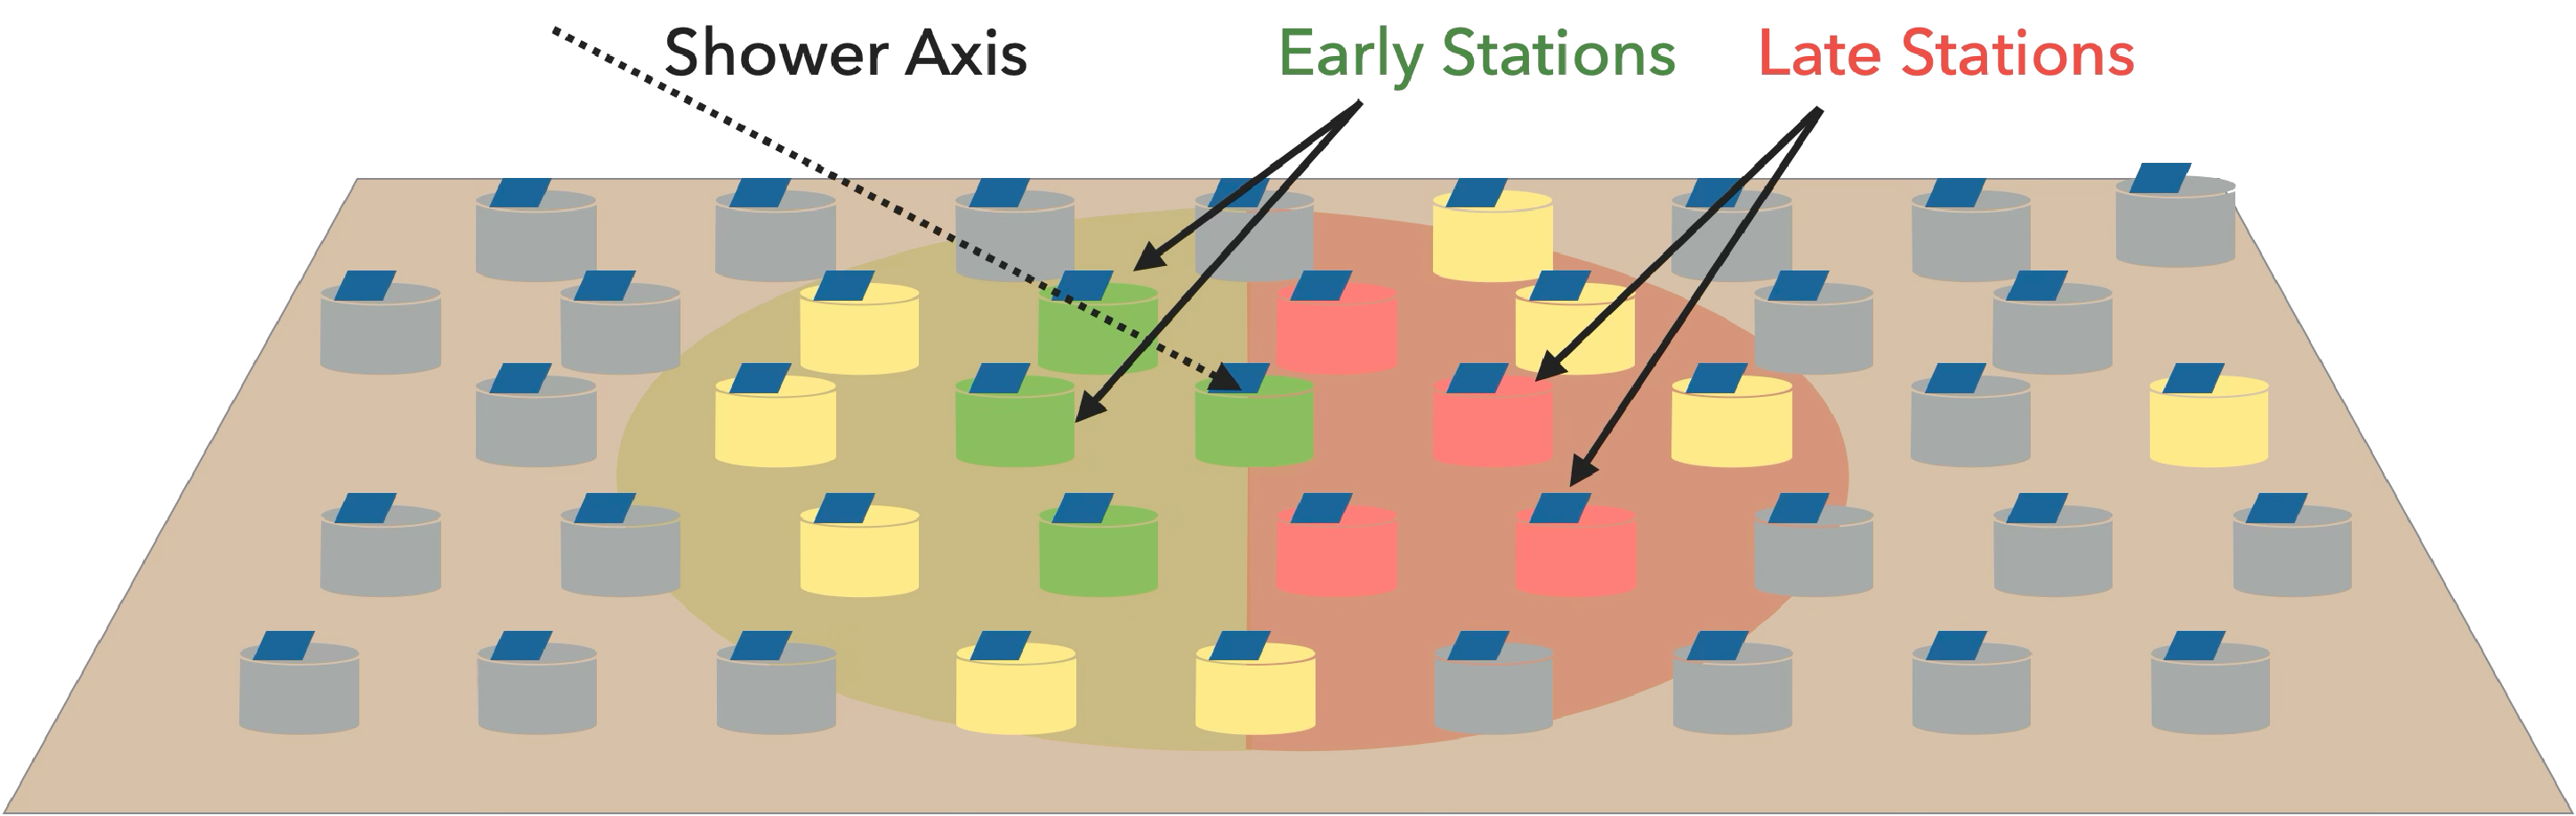
\includegraphics[width=\textwidth]{thesis_figures/Nu_analysis/Fisher_early_late.pdf}
  \caption{An illustration to depict the station selection process for the Fisher polynomial. The AoPs of the green stations are used to build the Fisher polynomial i.e. stations triggered earliest in the first crown. Stations in yellow are the ones triggered by the EAS and take part in the shower reconstruction.}
  \label{fig:AoP_early_late}
\end{figure}

Different forms of the Fisher polynomial were tested, and their performance was evaluated based on the MC neutrinos passing the evaluated Fisher cut which described in the next section. In this section only two forms are mentioned, the baseline polynomials were taken to be the one described in the previous analysis~\cite{gap_note_2013} and the final one used for this analysis. For the first three angular regions (58.5$^\circ \leq \theta < 67.5^\circ$) a more stringent criterion which requires the AoPs of the first five triggered T5 stations was used to build the Fisher polynomial. For the remaining two angular regions (67.5$^\circ \leq \theta < 76.5^\circ$) only the first four triggered T5 stations were required. The form of the Fisher polynomial used in the previous analysis is given below:

\begin{equation}
  \mathcal{F} = \sum_{i=1}^{4or5} C_i AoP_i + C_p \prod_{i=1}^{4or5} AoP_i
\end{equation}

where $C_i$ and $C_p$ are the corresponding Fisher coefficients. 

A modified version of this baseline polynomial was used for this analysis. The product term was found to not have a significant contribution to the separation and was thus removed for this analysis. Further, the requirement of five stations for lower angular regions was also eliminated which effectively lowered the minimum number of stations required for each event. The form of the polynomial used is : 
\begin{equation}
  \label{eq:fisher_poly_new}
  \mathcal{F} = \sum_{i=1}^{4} C_i AoP_i
\end{equation}

The performance comparison of the two polynomials which is also the overall is discussed in the next section.

As mentioned before to train the Fisher polynomial 20\% of the measured data sample for the time period 2014-2021 as the background training sample. Since this is measured data at the detector it is already weighted by energy (cross-section is a function of primary energy) and zenith angle (affects available detection area). For the MC neutrino events (signal sample) which do not have this natural weighting, each event is weighted by a factor of $\omega = E_{MC}^{-1} \cdot \sin(\theta_{MC}) \cdot \cos(\theta_{MC})$. The fig~\ref{} shows the Fisher value, $mathcal{F}$ distributions for both signal and background training distributions for all five angular regions. An excellent separation is achieved for all angular regions. 

\subsubsection{Fisher Cut and background estimation}
\label{subsubsec:nu_sel_fisher_cut}
After the training process a cut criterion is still needed to be established to best separate the signal and background distribution. This cut is evaluated by analysing the tail of the Fisher value distribution of the background. 

The tail is fit using an exponential function in the logarithmic scale ($A \mathcal{F} + B$). The fitting is done between for the range $\mu + \sigma$ - $\mu + n\sigma$ where $\mu$ is the mean and $\sigma$ is the rms value of the distribution. n takes a value depending on the last non-zero angular bin for that region. The exponential assumption is only a reasonable guess especially due to the low statistics of the last few bins. The bin size can also affect the fit and is determined for each angular region by minimising the residual fit. This bin size is also verfied with the calculator available in python to negate the possibility of over binning or under binning. Table~\ref{} shows the \textit{observed} and \textit{predicted} values for the exponential fit procedure. The values are calculated by integrating from the start point mentioned in the first column till the end of the $\mathcal{F}$ distribution. The estimate using the exponential fit mostly agrees with the observed values. It agrees the best near the mean of the distribution and becomes worse near the tails. In some angular regions a secondary bump like structure is also seen. This is attributed to the form of the Fisher polynomial and the lack of the product term. The predicted values also include the uncertainties of the fit which slightly increases the predicted number of the background events. The cut, $\mathcal{F}_cut$ is calculated such that after 20 years of data taking with a full SD array 0.2 events are expected to pass for each sub-angular regions with a total of 1 background event for the full search angular range. 

\begin{equation}
  \mathcal{F}_{cut} = \mathrm{\frac{log[1.25 \cdot B \cdot 0.2 \cdot \Delta (\mathcal{F}) / 20] - A}{B} }
\end{equation}

The two polynomials mentioned in the above section are evaluated based on the fraction of neutrino events passing the $\mathcal{F}_{cut}$. As can be seen in fig.~\ref{}. The simplified Fisher polynomial either matches or outperforms the polynomial used in the previous analysis. The comparison is done only for the case where new triggers are included. The much higher number of events in this sample are required to achieve a sufficiently high background-signal separation especially in the low zenith angular regions where previously a more stringent number of station cut was needed to reduce noise. However, the new Fisher polynomial seems to perform even better for higher angles which could lead to an overall improvement of neutrino detection efficiency irrespective of energy. This is proved later in sec.~\ref{sec:det_exposure_calc}. Based on this comparison the polynomial given in~\ref{eq:fisher_poly_new} was used for signal-background separation is this analysis. 

Fig~\ref{} shows the $\mathcal{F}_{cut}$ obtained for the different angular regions. 

A two-dimensional plot with the Fisher values on an event by event basis vs the zenith angle is shown in fig~\ref{}. The blue dots represent the background events and the contour represents the signal events. The black line is obtained by setting the $\mathcal{F}_{cut}$ to the mid value of the bin and the extrapolating for a particular sub-angular region. The background events seem to be distributed non-uniformally within the angular subsamples. The linear interpolation ensures that the effective number of events is almost constant with the zenith angle. Anything above the cut line will be considered as a neutrino candidate. 

\begin{table}[h!]
  \centering
  \begin{tabular}{ |P{1.25cm}||P{2.4cm}|P{2.4cm}|P{2.4cm}|P{2.4cm}|P{2.4cm}| }
    \hline
      Fit & \multicolumn{5}{c|}{Number of events in $\mathcal{F}$ tails} \\
      Range & \multicolumn{5}{c|}{Observed - Predicted} \\
    \cline{2-6}
      & Region 1 & Region 2& Region 3& Region 4 & Region 5 \\
      &(58.5$^\circ$-61.5$^\circ$]&(61.5$^\circ$-64.5$^\circ$]&(64.5$^\circ$-67.5$^\circ$]& (67.5$^\circ$-70.5$^\circ$] & (70.5$^\circ$- 76.5$^\circ$] \\
    \hline 
    $\mu$ + 1$\sigma$ & 13 & 14 & 17 & 19 & 23 \\
    $\mu$ + 2$\sigma$ & 1640 & 1820 & 2040 & 2330 & 2720 \\
    $\mu$ + 3$\sigma$ & 140 & 220 & 140 & 230 & 120 \\
    $\mu$ + 4$\sigma$ & 140 & 220 & 140 & 230 & 120 \\
    $\mu$ + 5$\sigma$ & 140 & 220 & 140 & 230 & 120 \\
    $\mu$ + 6$\sigma$ & 140 & 220 & 140 & 230 & 120 \\
    \hline
  \end{tabular}
  \caption{Table to test captions and labels.}
  \label{tab:Cut_eval}
\end{table}

\begin{table}[h!]
  \centering
  \begin{tabular}{ |P{2.5cm}||P{2.3cm}|P{2.3cm}|P{2.3cm}|P{2.3cm}|P{2.3cm}| }
    \hline
      \multicolumn{6}{|c|}{$\nu$ selection summary} \\
      \hline
      \multirow{3}{*}{\shortstack{Inclined Sel.\\ $\theta_{rec} \in$}} & Region 1 & Region 2& Region 3& Region 4 & Region 5 \\
            &(58.5$^\circ$-61.5$^\circ$]&(61.5$^\circ$-64.5$^\circ$]&(64.5$^\circ$-67.5$^\circ$]& (67.5$^\circ$-70.5$^\circ$] & (70.5$^\circ$- 76.5$^\circ$] \\
      \cline{2-6}      
            & \multicolumn{5}{c|}{$\delta \theta_{rec} < 3^{\circ}$} \\ 
    \hline
    Fiducial Quality & \multicolumn{5}{c|}{6T5} \\
    \hline
    Young Shower Sel. & \multicolumn{5}{c|}{75 \% of T5 stations to be ToT/ToTd/MoPS} \\
    \hline
    Angular Fit Quality & \multicolumn{5}{c|}{$\chi^2/ndof < 200$} \\
    \hline
    \multirow{2}{*}{\shortstack{Fisher Discrim.\\ $\mathcal{F}$}} & \multicolumn{5}{c|}{$\sum_{i=1}^{4} C_i AoP_i$} \\
       & \multicolumn{5}{c|}{i = number of first T5 triggered stations} \\ 
    \hline
    ($\theta, \mathcal{F}_{cut}$) &(60,) & (63,) & (66,) & (69,) & (73.5,) \\
    \hline
  \end{tabular}
  \caption{Table to test captions and labels.}
  \label{tab:Selection_summ}
\end{table}

\subsection{Time evolution of selection parameters}
\label{subsec:nu_sel_timeev}

A time evolution study of the selection parameters used in the $\nu$ analysis is very important as any missed non-physical phenomenon which impacted data taking with the SD can erroneously affect the training procedure. Since the search sample is kept "blind" and the analysis is fixed based on the training samples, any missed error during the training procedure could result in fake neutrino candidates when the search sample is unblinded. 

The first step that is taken to mitigate such instances is in the way the background training sample is chosen. Since the 20\% background sample is chosen randomly over the same time period as that of the search sample it already should be a good representative of the search sample. The check is still performed to look for specific features for the selection parameters such as AoP, Fisher value, Long signal fraction and the zenith angle. 

The values for these parameters is plotted vs the SD Event ID which is correlated to time and represents the time evolution of the array. Fig~\ref{} shows the evolution of the Long signal fraction with respect to the SD Event ID number. The Long signal fraction is likely to be time dependent~\cite{Sato:2011zze} as the signal threshold for the triggers can be affected by changes in the SD stations (PMT degradation, change in linear reflectivity etc.). There is an ongoing effort to include the affect of ageing of the detector for future detector simulations~\cite{PierreAuger:2023xfj}. Since, this work is still ongoing it was not used for this analysis. 

Fig~\ref{} show the evolution of AoP of the stations and the value of the Fisher discriminant with respect to the SD Event ID. AoP shows a slight modulation which could be related to the effect mentioned in~\cite{Sato:2011zze} and was also observed in the previous DG$\mathrm{_{low}}$ analysis. This modulation was also observed to have a slight zenith angle dependence as shown in the figure. Overall, this effect is very small and is not expected to affect the analysis.

\subsection{Neutrino Detection Efficiency}
\label{subsec:nu_sel_nudeteff}

In this section, the detection efficiency at each stage of the $\nu$ selection procedure is identified. The efficiency is affected by a myraid of factors such as neutrino flavour, NC or CC interaction, energy, zenith angle and slant depth of interaction. The list is presented in table~\ref{tab:Selection_eff}. The numbers are calculated with respect to the events remaining after the precedent cut. They are presented sequentially ordered according to the application of the cut in the selection chain. The values are obtained from MC simulations assuming a fully functional surface detector array. 

\begin{table}[h!]
  \centering
  \begin{tabular}{ |P{3cm}||P{4cm}|P{1.5cm}|P{1.5cm}| }
    \hline
      \multicolumn{4}{|c|}{$\nu$ selection efficiencies} \\
      \hline
      \multicolumn{2}{|c|}{Cut} & \multicolumn{2}{c|}{Efficiency} \\
      \cline{3-4}
      \multicolumn{2}{|c|}{} & CC & NC \\
      \hline      
      Inclined Selection & 58.5$^\circ < \theta_{rec} \geq 76.5^{\circ}$ & 90\% & 96\% \\ 
    \hline
    Fiducial Quality & 6T5 & 90\% & 96\%\\
    \hline
    Young Shower Selection & 75 \% of T5 stations to be ToT/ToTd/MoPS & 90\% & 96\% \\
    \hline
    Angular Fit Quality & $\mathrm{\chi^2/ndof < 200}$ & 90\% & 96\% \\
    \hline
    \multirow{2}{*}{Station Cut } & No. of T5 & 90\% & 96\% \\
                                            & triggered stations $\geq 4$ & & \\ 
    \hline
    Neutrino Selection & $\mathcal{F}_{\mathrm{cut}}$ & 90\% & 96\%\\
    \hline
  \end{tabular}
  \caption{Table to test captions and labels.}
  \label{tab:Selection_eff}
\end{table}

The inclined shower selection removes $\sim x\%$ of showers. These showers were previously discussed in section~\ref{sec:reco_possel}. Most of these events are showers which interact very close to the ground which can lead to a mis-reconstructed zenith angle. Further, calculating the impact of $\Delta \theta_{rec}$ a stronger reduction is observed in NC than CC events. The error distributions for both channels are given in fig~\ref{}. The error seems to worsen with increasing zenith angle and reduction of shower energy. These are the two areas where the reconstruction algorithm does not perform properly as in both cases the number of triggered stations are very few and additionally in the second case certain geometrical patterns such as a line can impact the zenith angle determination.

The fiducial quality cut is already a part of the reconstruction algorithm and is thus not evaluated in this section.

The long signal trigger fraction impact \todo{Write more after the numbers}

It is also observed that the Fisher discrimination has different efficiency based on the channel. It seems to perform better for the CC channel in comparison to the NC channel. This is further analysed by looking at the AoP distribution for the two channels in fig.~\ref{}. On average the CC events have a higher AoP value in comparison to the NC events. The values of AoP for NC lie in between the CC and the background events. This makes for a less efficient separation for the NC channel. Overall NC channel events seems to retain a lower electro magnetic component when they reach the ground in comparison to the CC events. This was already shown in the previous analysis.

Fig~\ref{} shows the comparison of the neutrino detection efficiency w.r.t. the zenith angle for the CC channel at different primary energies. The plot is compared to the one shown in the previous analysis. Overall the efficiency increases with energy reached maximum values for $\sim 10^{20.5}$. The efficiency increases as a function of zenith angle with a maximum efficiency for $\theta_{MC} \sim 70^{\circ}$. The efficiency slightly decreases for angles above $ \sim 73^{\circ}$, since for very inclined showers the electromagnetic component at ground is significantly less, which affects the identification efficiency. Another factor contributing to this decrease for higher zenith angles is the quality cut on $\Delta \theta_{rec}$ which disproportionally affects the highest zenith angles since the angular reconstruction algorithm is not optimized for very inclined showers. 

It was observed that by using the new triggers a 500-200\% improvement can be achieved for the neutrino search for the DG$\mathrm{_{low}}$ channel especially for the CC channel. The effect of the improvement decreases for higher energy and is the most prominent for energies up to $log E_{\nu} = 18.5$eV. There are several effects which contribute to this improvement. The new triggers increase the overall number of events especially for lower energies as shown in fig~\ref{}. The other factors which are different in this analysis is the reduction of the minimal T5 station requirement for the low angular regions and the change of the Fisher polynomial also contribute to the overall neutrino detection improvement in comparison to the previous analysis. A similar behaviour is observed for the NC channel albeit with a reduced overall efficiency in comparison to the CC channel. 





\begin{figure}[t!]
\centering
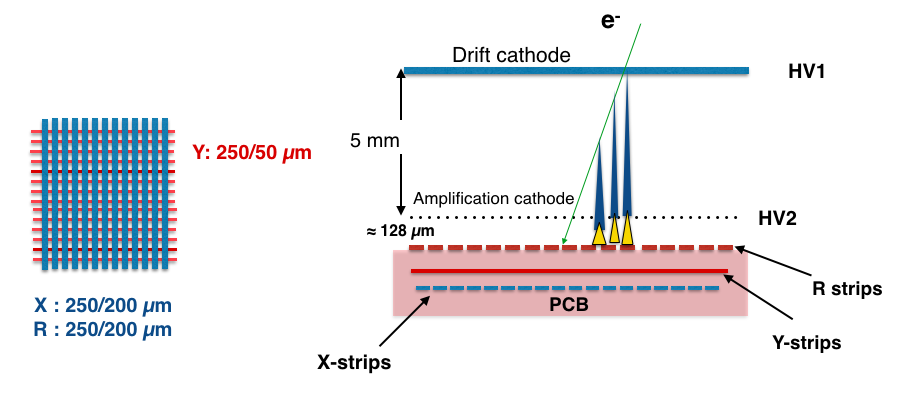
\includegraphics[width=\textwidth]{thesis_figures/NA64_MM.png}
\caption{Left: Strip dimensions of the modules, Right:NA64 Micromega's working principle~\cite{}}
\label{fig:Micromegas_na64}
\end{figure}

\begin{figure}[t!]
\centering
  \begin{minipage}[t]{.45\textwidth}
    \centering
    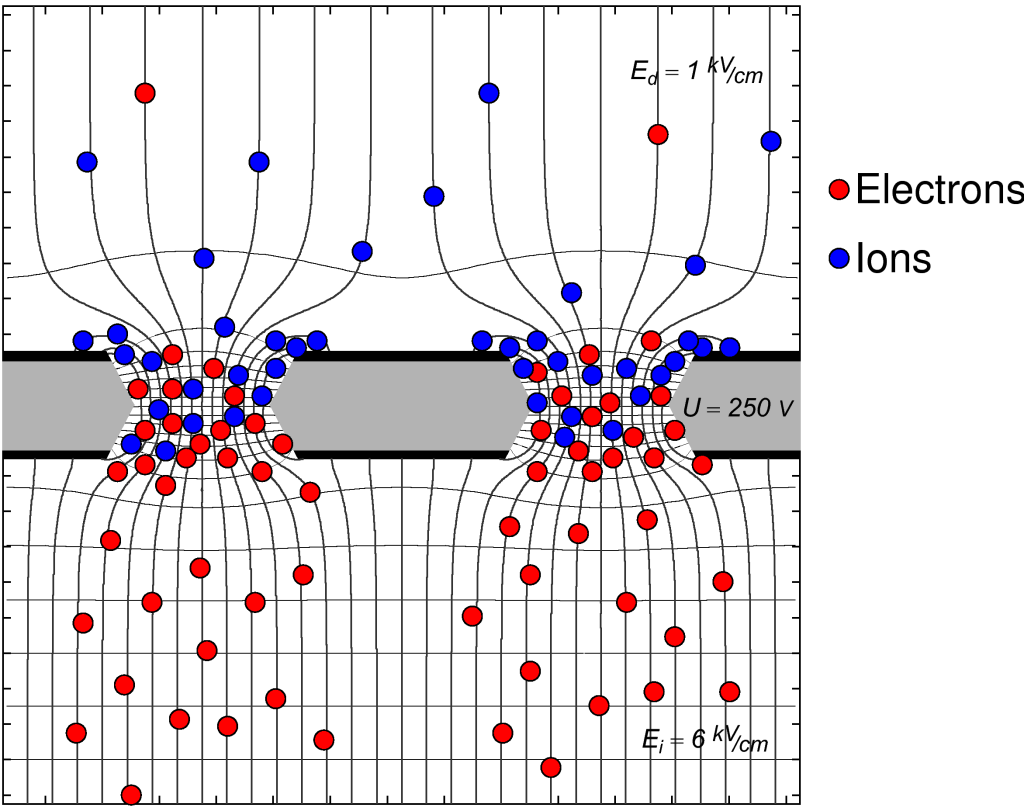
\includegraphics[width=\linewidth]{thesis_figures/GEM_field.png}

    \caption{A sketch of GEM field lines~\cite{}.}
    \label{fig:GEM_field}
  \end{minipage}
  \hfill
  \begin{minipage}[t]{.45\textwidth}
    \centering
    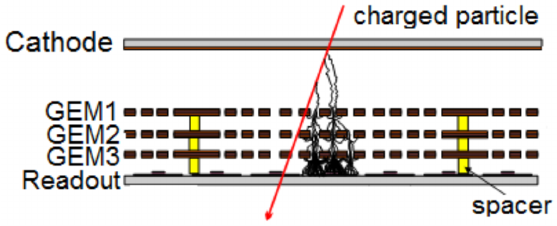
\includegraphics[width=\linewidth]{thesis_figures/GEM_process.png}
    \caption{Schematic of a triple GEM detector along with the working principle~\cite{}}
    \label{fig:Triple_GEM}
  \end{minipage}
\end{figure}
\begin{figure}[t!]
\centering
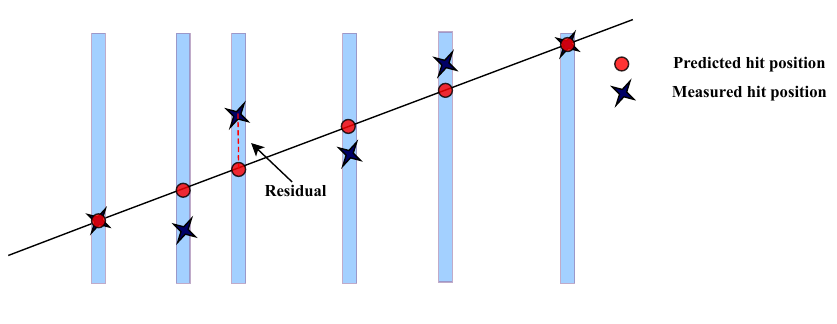
\includegraphics[width=\textwidth]{thesis_figures/linear_reg_new.png}
\caption{Linear regression pictorially. }
\label{fig:linear_regression}
\end{figure}



%%% Local Variables:
%%% mode: latex
%%% TeX-master: "mythesis"
%%% End:
